\documentclass[
	aspectratio=169, % default is 43
	8pt, % font size, default is 11pt
	handout, % handout mode without animations, comment out to add animations
]{beamer}

\documentclass[
	aspectratio=169, % default is 43
	8pt, % font size, default is 11pt
	handout, % handout mode without animations, comment out to add animations
]{beamer}

\usepackage{../template/beamerthemeuulm} % use the inofficial uulm beamer theme
\setfaculty{infIngPsy} % set the color scheme for your faculty here [med/infIngPsy/math/nat]

% requires symbolic links
% git clone git@github.com:SoftVarE-Group/SlideTemplate.git C:\Users\...\SlideTemplate
% mklink /J template C:\Users\...\SlideTemplate
% git clone git@spgit.informatik.uni-ulm.de:thuem/slides.git C:\Users\...\ThomasSlides
% mklink /J thomasslides C:\Users\...\ThomasSlides
\graphicspath{{../template/pics/logos}{../template/pics/nature}{../template/pics/uulm}{../thomasslides/}{../pics/people/}{../pics/xkcd/}}

%\usepackage[ngerman]{babel} % use this line for slides in German
%\recordingtrue % special recording mode for use with a greenscreen, gives you space to show yourself in a layer in front of the slides, has no effect in the handout mode

\title{Software Product Lines} % short title is used for the slide footer but optional

% LINKED LITERATURE

\newcommand{\ludewiglichter}{\href{https://learning.oreilly.com/library/view/-/9781457184932/?ar}{Ludewig and Lichter}}
\newcommand{\seeconomics}{\href{https://rds-ulm.ibs-bw.de/link?kid=027381854}{SE Economics}}
\newcommand{\sommervillelink}[1]{\href{https://ulm.ibs-bw.de/aDISWeb/app?service=direct/0/Home/$DirectLink\&sp=SOPAC00\&sp=SAKSWB-IdNr1615420983}{#1}}
\newcommand{\sommerville}{\sommervillelink{Sommerville}}
\newcommand{\thehumbleprogrammer}{\href{https://dl.acm.org/doi/10.1145/1283920.1283927}{The Humble Programmer}}
\newcommand{\thepragmaticprogrammer}{\href{https://learning.oreilly.com/library/view/the-pragmatic-programmer/9780135956977/}{The Pragmatic Programmer}}

% TYPICAL COMMANDS FOR LECTURES

\renewcommand{\emph}[1]{{\color{blue}\textbf{#1}}}

\newcommand{\deutsch}[1]{{\color{blue}(#1)}}
\newcommand{\deutschertitel}[1]{{\tiny\deutsch{#1}}}

\newcommand{\mycite}[1]{``#1''}
\newcommand{\mytitlesource}[1]{{\tiny\normalfont\mbox{[#1]}}}
\newcommand{\mysource}[1]{\ifthenelse{\equal{#1}{}}{}{\phantom{.}~\hfill~\mytitlesource{#1}}}

\newcommand{\todo}[1]{{\color{red}\textbf{[#1]}}}
\newcommand{\fodo}[1]{\todo{\footnote{\todo{#1}}}}
\newcommand{\todots}{\todo{\ldots}}

% IMPORTED PACKAGES

%\usepackage{adjustbox} % used for partofpage
%\usepackage{tcolorbox} % used for mydefinition, mynote, myexample
\usepackage{multicol} % used temporarily for the lecture overview
\usepackage{mathtools} % required for absolute value in modeling lecture

% COMMANDS TO LAYOUT AND ANNIMATE SLIDES

\newcommand{\lessonslearned}[3]{
	\subsection{Summary}
	\begin{frame}{\insertsection -- \insertsubsection}
		\leftorright{
			\mydefinition{Lessons Learned}{
				\begin{itemize}
					#1
				\end{itemize}
			}
			\mynote{Further Reading}{
				\small % references take space, can be a little smaller
				\begin{itemize}
					#2
				\end{itemize}
			}
		}{
			\myexample{Practice}{
				#3
			}
		}
	\end{frame}
}

% TODO temporary hack to layout the slide overview in two colums
\renewcommand{\lectureoverview}{
%	\section*{Overview}
%	\subsection*{Overview}
	\begin{frame}{\insertsubtitle}
		\begin{multicols}{2}
			\tableofcontents
		\end{multicols}
	\end{frame}
}

\renewcommandx{\maketitle}[2][1=apr21-o25a,2=150]{
    {
	\usebackgroundtemplate{} % TODO temporary hack to enable missing pictures at title slide
	%\ifx {#1} \empty \else {\usebackgroundtemplate{\includegraphics[trim=0 0 0 #2,clip,width=\paperwidth]{#1}}} \fi     
	%\usebackgroundtemplate{\includegraphics[trim=0 0 0 #2,clip,width=\paperwidth]{#1}}
    \begin{frame}[plain]
        \vskip0pt plus 1filll
        \begin{beamercolorbox}[wd=\paperwidth,ht=4.5ex,dp=2ex,right]{titlebox}
            \LARGE\textbf{\inserttitle}\hspace*{20pt}
        \end{beamercolorbox}%
        \nointerlineskip%
        \begin{beamercolorbox}[wd=\paperwidth,ht=2.25ex,dp=1ex,right]{subtitlebox}
            \small 
            \ifx \insertsubtitle \empty \else \insertsubtitle\ $\vert$ \fi
            \insertauthor\
            \ifx \insertdate \empty \else $\vert$ \insertdate \fi
            \hspace*{20pt}
        \end{beamercolorbox}%
        \nointerlineskip%
        \begin{beamercolorbox}[wd=\paperwidth,ht=4.5ex,dp=2ex,left]{logobox}
            \centering
            \vspace{-1ex}
            \hspace{10pt}
            \includegraphics[height=4.5ex]{sp} % SPECIFY INSTITUTE LOGO HERE
            \hfill
            \includegraphics[height=4.5ex]{uulm}
            \hspace{10pt}
        \end{beamercolorbox}%
    \end{frame}
    }  
}

%
%\newcommand{\onlyleft}[1]{
%	\halfpage{#1}
%}
%
%\newcommand{\onlyright}[1]{
%	~\hfill
%	\halfpage{#1}
%}
%
%\newcommand{\leftorright}[2]{
%	\uncover<1>{\halfpage{#1}}
%	\hfill
%	\uncover<3->{\halfpage{#2}}
%}
%
%\newcommand{\rightorleft}[2]{
%	\uncover<3->{\halfpage{#1}}
%	\hfill
%	\uncover<1>{\halfpage{#2}}
%}
%
%\newcommand{\leftthenright}[2]{
%	\halfpage{#1}
%	\hfill\pause
%	\halfpage{#2}
%}
%
%\newcommand{\leftandright}[2]{
%	\halfpage{#1}
%	\hfill
%	\halfpage{#2}
%}
%
%\newcommand{\leftmiddleandright}[3]{
%	\thirdpage{#1}
%	\hfill
%	\thirdpage{#2}
%	\hfill
%	\thirdpage{#3}
%}
%
%\newcommand{\leftmiddleorright}[3]{
%	\uncover<1>{\thirdpage{#1}}
%	\hfill
%	\uncover<3>{\thirdpage{#2}}
%	\hfill
%	\uncover<5->{\thirdpage{#3}}
%}
%
%\newcommand{\halfpage}[1]{\partofpage{48}{#1}}
%
%\newcommand{\thirdpage}[1]{\partofpage{31}{#1}}
%
%\newcommand{\partofpage}[2]{
%	\adjustbox{valign=t}{\begin{minipage}{0.#1\textwidth}
%			\begin{flushleft}
%				#2
%			\end{flushleft}
%	\end{minipage}}
%}
%
%\newcommand{\mydefinition}[2]{
%	\begin{tcolorbox}[title=#1,colback=orange!10,colframe=orange!30,coltitle=black,fonttitle=\bfseries,left=1mm,right=1mm,top=1mm,bottom=1mm]
%		\begin{flushleft}
%			#2
%		\end{flushleft}
%	\end{tcolorbox}
%}
%
%\newcommand{\mydefinitiontight}[2]{
%	\begin{tcolorbox}[title=#1,colback=white,colframe=orange!30,coltitle=black,fonttitle=\bfseries,left=0mm,right=0mm,top=0mm,bottom=0mm]
%		\begin{flushleft}
%			#2
%		\end{flushleft}
%	\end{tcolorbox}
%}
%
%\newcommand{\mynote}[2]{
%	\begin{tcolorbox}[title=#1,colback=red!10,colframe=red!30,coltitle=black,fonttitle=\bfseries,left=1mm,right=1mm,top=1mm,bottom=1mm]
%		\begin{flushleft}
%			#2
%		\end{flushleft}
%	\end{tcolorbox}
%}
%
%\newcommand{\myexample}[2]{
%	\begin{tcolorbox}[title=#1,colback=blue!10,colframe=blue!30,coltitle=black,fonttitle=\bfseries,left=1mm,right=1mm,top=1mm,bottom=1mm]
%		\begin{flushleft}
%			#2
%		\end{flushleft}
%	\end{tcolorbox}
%}
%
%\newcommand{\myexampletight}[2]{
%	\begin{tcolorbox}[title=#1,colback=white,colframe=blue!30,coltitle=black,fonttitle=\bfseries,left=0mm,right=0mm,top=0mm,bottom=0mm]
%		\begin{flushleft}
%			#2
%		\end{flushleft}
%	\end{tcolorbox}
%}

% SET UNIVERSITY
% \berntrue
% \magdeburgtrue
% \ulmtrue

% Tables
\usepackage{booktabs}

\subtitle{2. Runtime Variability and Design Patterns}
\author{Timo Kehrer, Thomas Thüm, Elias Kuiter}
\foruniversity{}
	{\setpicture[300]{magdeburg-canal}}
	{\setpicture{oct20-south4}}

\begin{document}

\mode<handout>{\contentoverview}

\mode<beamer>{
	\ifdefined\thepicture
		\maketitle[\thepicture][\thepictureoffset]
	\else
		\maketitle[]
	\fi
}

% shared slide content

% introduced: 02a-configuration
% reused: 03a-intro
\newcommand{\frameImplementSPLs}{
	\begin{mycolumns}[widths={45},animation=none]
		\pic[width=\linewidth]{metaproduct2}
	\mynextcolumn
		\begin{note}{Key Issues}
			\begin{itemize}
			\item Systematic reuse of implementation artifacts
			\item Explicit handling of variability
			\end{itemize}
		\end{note}
		\uncover<2->{\begin{definition}{Variability\mysource{\fospl\mypage{48}}}
			\mycite{\emph{Variability} is the ability to derive different products from a common set of artifacts.}
		\end{definition}}
		~
		\uncover<3->{\begin{note}{Variability-Intensive System}
			Any software product line is a variability-intensive system. % TODO Timo: do we really need this term? where does this definition come from?
		\end{note}}
	\end{mycolumns}
}

% introduced: 02a-configuration
% reused: 02b-implementation, 03a-intro
\newcommand{\frameVariabilityAndBindingTimes}{
	\begin{mycolumns}[widths={55},animation=none]
		\begin{definition}{Binding Time \deutsch{Bindungszeitpunkt}\mysource{\fospl\mypage{48}}}
			\begin{itemize}
				\item Variability offers choices
				\item Derivation of a product requires to make decisions (aka. binding)
				\item Decisions may be bound at different binding times
			\end{itemize}
		\end{definition}
		~
		\uncover<2->{\begin{note}{When? By whom? How?}
			\lectureruntime\parta: \emph{when} and \emph{by whom}

			\lectureruntime\partb: \emph{how}
		\end{note}}
	\mynextcolumn
		\pic[width=\linewidth]{metaproduct2}
	\end{mycolumns}
}

% introduced: 03a-intro
% reused: 03a-intro
\newcommand{\frameRuntimeVariabilityProblems}{
	\begin{note}{Problems of Runtime Variability}
		{\bf Conditional Statements:}
		\begin{itemize}
			\item Code scattering, tangling, and replication
		\end{itemize}
		{\bf Design Patterns for Variability:}
		\begin{itemize}
			\item Trade-offs and potential negative side effects
			\item Constraints that may restrict their usage
		\end{itemize}
		{\bf In General:}
		\begin{itemize}
			\item Variable parts are always delivered
			\item Not well-suited for compile-time binding
		\end{itemize}
	\end{note}
}

% introduced: 03a-intro
% reused: 03a-intro
\newcommand{\frameSoftwareConfigurationManagement}{
	\begin{mycolumns}
		\begin{definition}{Software Configuration Management} % TODO source missing
			Policies, processes, and tools for managing evolving software systems:
			\begin{itemize}
				\item Version control
				\item System building
				\item Release management
				\item Change management
				\item Collaborative work
			\end{itemize}
		\end{definition}
	\mynextcolumn
		\begin{note}{No Software Configuration Management}
			\lecturecloneandown\parta: Ad-Hoc Clone-and-Own

			aka.\ unmanaged clone-and-own
		\end{note}
		\begin{note}{Version Control}
			\lecturecloneandown\partb: Clone-and-Own with Version Control

			instance of managed clone-and-own
		\end{note}
		\begin{note}{System Building}
			\lecturecloneandown\partc: Clone-and-Own with Build Systems

			instance of managed clone-and-own
		\end{note}
	\end{mycolumns}
}


% runtime variability
%   input: flags in source code, configuration files, runtime parameters (avoid recompilation)
%   realization: if, switch, encoded in objects/state, inheritance
%   design patterns for variability / OOP + outlook beyond runtime variability

\section{Configuration of Runtime Variability}

%\begin{frame}{Variants of Graphs and Their Features}
	%\centering
	%\includegraphics[width=.7\linewidth,page=6,trim=20 20 20 150,clip]{FeatureIDE with Graphs/2016-05-19 ICSE FeatureIDEdemo}
	%% TODO export into separate PDF containing only the separate products
%\end{frame}
%
%\subsection{Runtime Parameters}
%\begin{frame}{\myframetitle}
	%\leftorright{
		%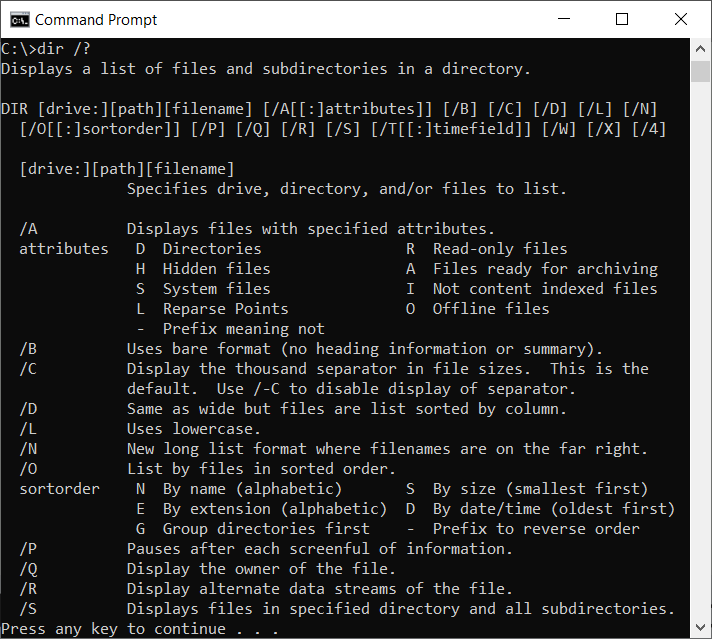
\includegraphics[width=\linewidth]{runtime-parameters-win10-cmd-dir}
	%}{
		%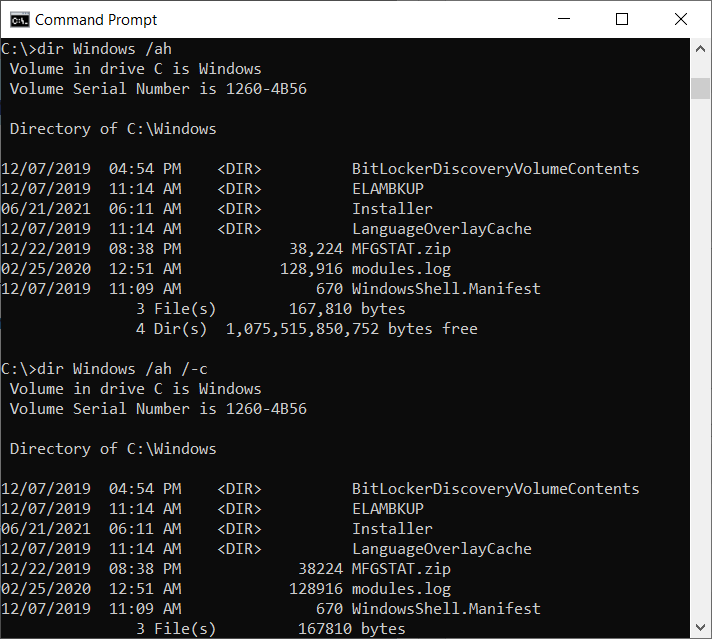
\includegraphics[width=\linewidth]{runtime-parameters-win10-cmd-dir2}
	%}
%\end{frame}

\begin{frame}{Recap: Software Product Lines}
	\begin{mycolumns}
		\mydefinition{Software Product Line \mysource{\seiwhitepaperspl\mypage{5}}}{\mycitebegin A \emph{software product line} is 
			\begin{itemize}
				\item a set of software-intensive systems (aka.\ products or variants)
				\item that share a common, managed set of features 
				\item satisfying the specific needs of a particular market segment or mission (aka.\ domain)
				\item and that are developed from a common set of core assets in a prescribed way.\myciteend
			\end{itemize}
			\mysource{\href{https://resources.sei.cmu.edu/library/asset-view.cfm?assetID=513819}{Software Engineering Institute, Carnegie Mellon University}}
		}
	\mynextcolumn
		\pic[width=\linewidth,page=24]{lego}
	\end{mycolumns}
\end{frame}

\subsection{Variability and Binding Time}

\begin{frame}{How to Implement Software Product Lines?}
	\begin{mycolumns}[widths={45},animation=none]
		
\includegraphics[width=\linewidth]{metaproduct2}	
	\mynextcolumn
		\mynote{Key Issues}{
			\begin{itemize}
			\item Systematic reuse of implementation artifacts.
			\item Explicit handling of variability.
			\end{itemize}
		}
		\uncover<2->{\mydefinition{Variability\mysource{\fospl\mypage{48}}}{
			Variability is the ability to derive different products from a common set of artifacts.
		}}
		~
		\uncover<3->{\mynote{Variability-Intensive System}{
			Any software product line is a variability-intensive system.
		}}
	\end{mycolumns}
\end{frame}

\begin{frame}{Variability and Binding Times}
	\begin{mycolumns}[widths={45},animation=none]
		
\includegraphics[width=\linewidth]{metaproduct2}	
	\mynextcolumn
		\mydefinition{Binding Time}{
			\begin{itemize}
				\item Variability offers choices.
				\item Derivation of a product requires to make decisions (aka. binding).
				\item Decisions may be bound at different binding times.
			\end{itemize}
		}	
		\uncover<2->{\mynote{When, how and by whom?}{
			In the sequel: Focus on when and by whom\ldots
		}}
	\end{mycolumns}
\end{frame}

\subsection{Command-Line Options}

\begin{frame}{Example: Command-Line Options}
	\leftorright{
		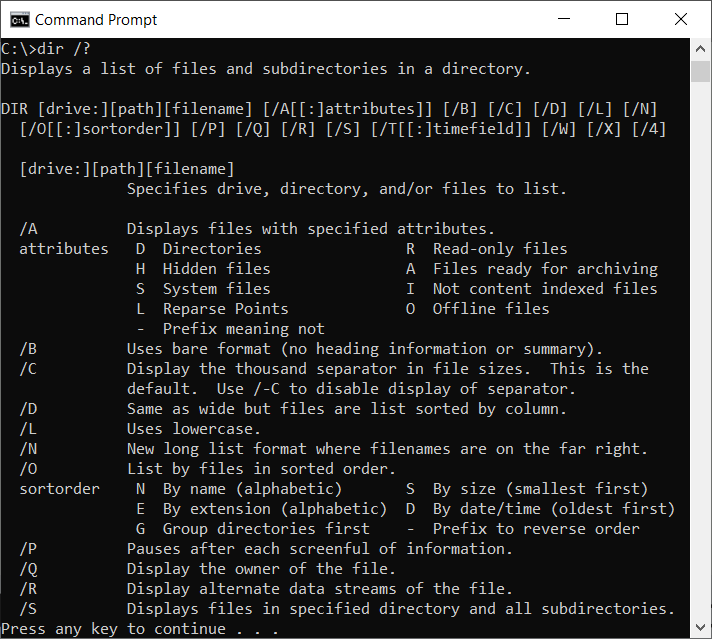
\includegraphics[width=\linewidth]{runtime-parameters-win10-cmd-dir}
	}{
		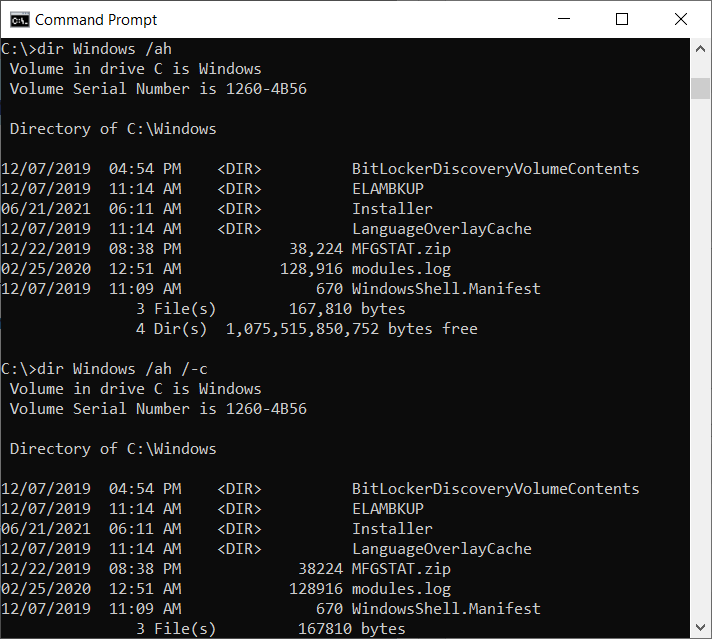
\includegraphics[width=\linewidth]{runtime-parameters-win10-cmd-dir2}
	}
\end{frame}

\subsection{Configuration Files}

\begin{frame}{Example: Configuration Files}
	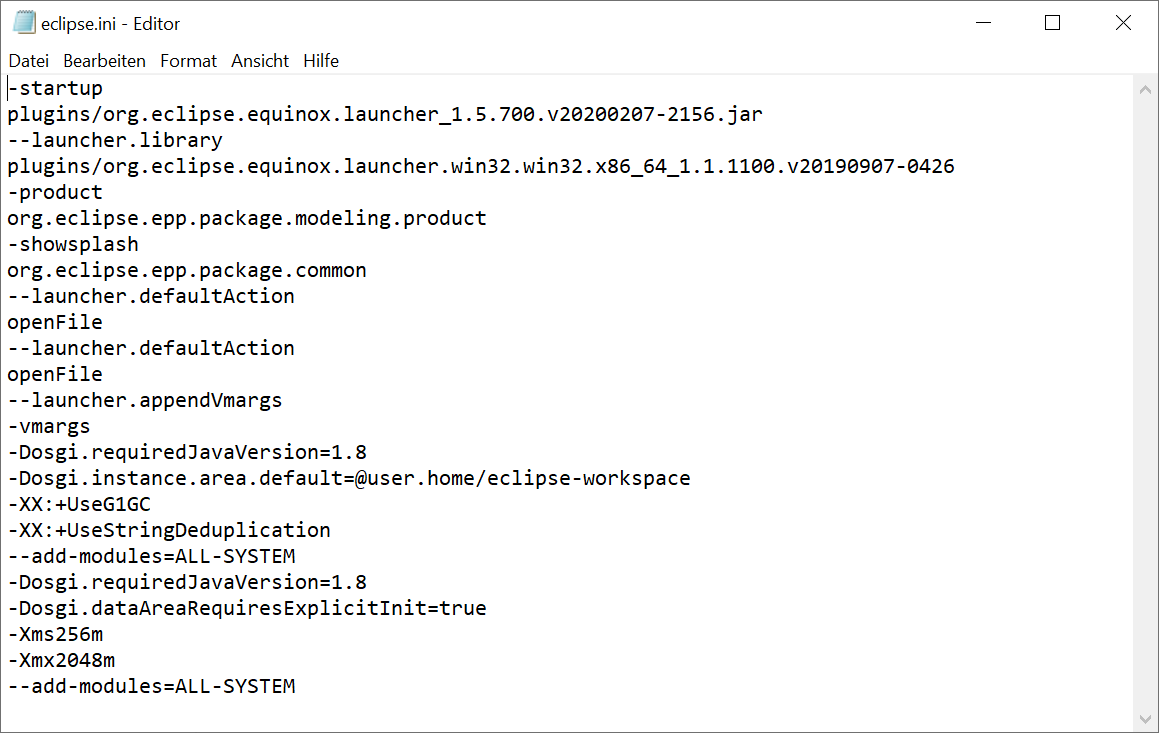
\includegraphics[width=0.75\linewidth]{configfile-eclipse-ini}
\end{frame}

\subsection{Preference Dialogs}

\begin{frame}{Example: Preference Dialogs}
	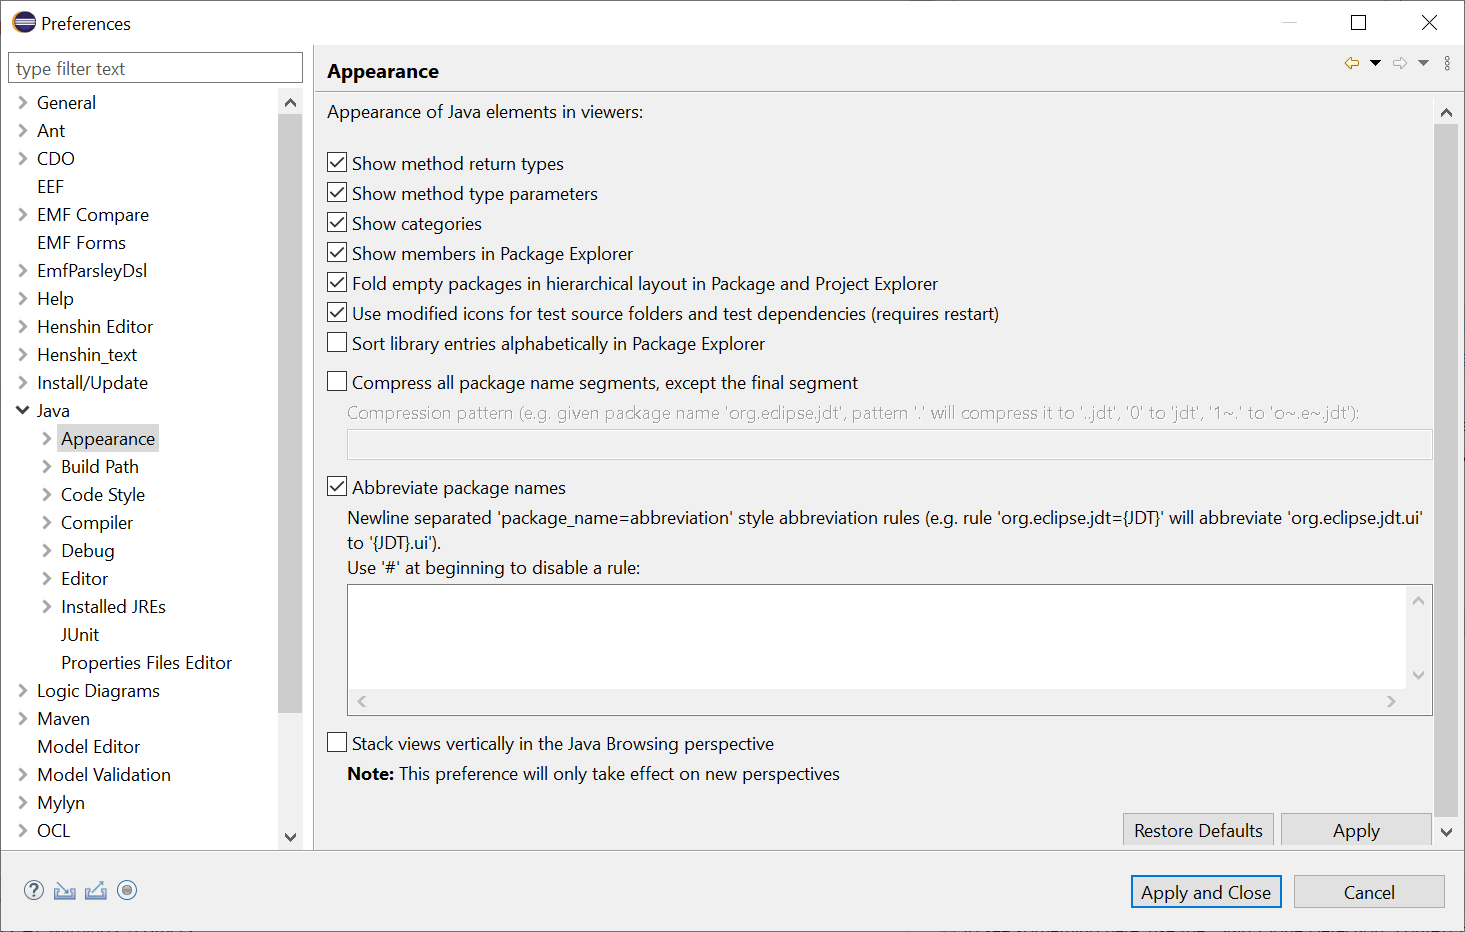
\includegraphics[width=0.75\linewidth]{preferences-eclipse}
\end{frame}

\subsection{Runtime Variability}

\begin{frame}{What do these examples have in common?}
	\begin{mycolumns}[columns=3,widths={26,36,36},animation=none]
		\pic[width=\linewidth]{runtime-parameters-win10-cmd-dir}
	\mynextcolumn
		\pic[width=\linewidth]{configfile-eclipse-ini}
	\mynextcolumn
		\pic[width=\linewidth]{preferences-eclipse}
	\end{mycolumns}
		
	\uncover<2->{
		\begin{mycolumns}[columns=2,widths={55,40},animation=none]
			\mynote{Configuration Parameters}{
				\begin{itemize}
					\item Behavior of a program is determined by configuration parameters being interpreted at runtime.
					\item In other words: Choices offered by variability are decided at runtime.
					\item Configuration may happen non-interactively (at startup) or interactively (through dialogs).
				\end{itemize}
			}			
		\mynextcolumn	
			\mydefinition{Runtime Variability\mysource{\fospl\mypage{49}}}{
				Runtime variability is decided after compilation when the program is started (aka. load-time variability) or during program execution.
			}	
		\end{mycolumns}
	}
\end{frame}

\subsection{Configuration Parameters}

\begin{frame}{Example: A Graph Library}
	A simple library providing \ldots \\
	\vspace{5mm}
	\leftorright{
		\myexample{\ldots graph data structures}{
			\begin{itemize}
				\item Directed/undirected edges
				\item Weighted/unweighted edges 
				\item Colored/uncolored nodes
				\item etc.
			\end{itemize}
		}		
	}{
		\myexample{\ldots and algorithms}{
			\begin{itemize}
				\item Vertex numbering
				\item Vertex coloring 
				\item Shortest path
				\item Minimum spanning tree 
				\item etc.
			\end{itemize}
		}
	}
\end{frame}

\begin{frame}{Features of a Graph}
	\begin{mycolumns}[columns=4,widths={25},animation=none]
		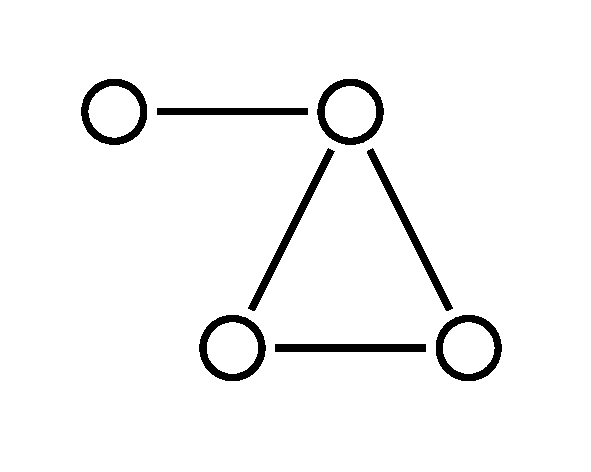
\includegraphics[width=\linewidth,page=1]{graphs}
		\includegraphics[width=\linewidth,page=3]{graphs}
		\ldots etc.
	\mynextcolumn
		\includegraphics[width=\linewidth,page=5]{graphs}
		\includegraphics[width=\linewidth,page=7]{graphs}
	\mynextcolumn
		\includegraphics[width=\linewidth,page=11]{graphs}
		\includegraphics[width=\linewidth,page=13]{graphs}
	\mynextcolumn
		\includegraphics[width=\linewidth,page=15]{graphs}
		\includegraphics[width=\linewidth,page=17]{graphs}		
	\end{mycolumns}
\end{frame}

\begin{frame}{Features as Configuration Parameters}
	\begin{mycolumns}[columns=3,widths={25,25,45},animation=none]
		\myexampletight{Directed}{\includegraphics[width=\linewidth,page=3]{graphs}}	
		\myexampletight{Colored}{\includegraphics[width=\linewidth,page=11]{graphs}}	
	\mynextcolumn
		\myexampletight{Weighted}{\includegraphics[width=\linewidth,page=5]{graphs}}	
		\myexampletight{Weighted, Colored}{\includegraphics[width=\linewidth,page=15]{graphs}}			
	\mynextcolumn
		\includegraphics[width=0.45\linewidth,page=6]{graphs}
		\hfill
		\includegraphics[width=0.45\linewidth,page=12]{graphs}
		
		~
		
		\mynote{Configuration of graph data structures}{
			\begin{itemize}
				\item Typically, configuration parameters are {\em flags}.
				\item Their boolean value determines which {\em features} are {\em activated} and which ones are {\em deactivated}.
			\end{itemize}
		}
	\end{mycolumns}
\end{frame}

\subsection{Validity of Parameter Settings}

\begin{frame}{\myframetitle}
	\begin{mycolumns}[columns=4,widths={65,5,15,15},animation=none]
		\begin{tabular}{llll}
			\toprule
			{\bf Algorithm} 							& {\bf Graph type} 	& {\bf Weights} & {\bf Coloring}  \\ \midrule
			{\em Vertex numbering}			  & *          				& *        			& *         			\\
			{\em Vertex coloring}       	& undirected 				& *        			& colored   			\\
			{\em Shortest path}        		& directed   				& weighted 			& *         			\\
			{\em Minimum spanning tree} 	& undirected 				& weighted 			& *         			\\
			\ldots         					& \ldots 			 			& \ldots 		  	& \ldots 					\\ \bottomrule
		\end{tabular}
		\vspace{5mm}	
		\uncover<2->{\mynote{Dependencies between features must be checked}{
			\begin{itemize}
				\item When the parameters are configured at startup, or
				\item whenever parameters are changed at runtime.
			\end{itemize}
		}}
	\mynextcolumn
		~
	\mynextcolumn
		\myexampletight{Directed}{\includegraphics[width=\linewidth,page=3]{graphs}}	
		\myexampletight{Colored}{
			\hfill\\
			\hfill\\
			\includegraphics[width=\linewidth,page=11]{graphs}
		}	
	\mynextcolumn
		\myexampletight{Weighted}{\includegraphics[width=\linewidth,page=5]{graphs}}	
		\myexampletight{Weighted, Colored}{\includegraphics[width=\linewidth,page=15]{graphs}}	
	\end{mycolumns}
\end{frame}

\lessonslearned{
	\item External setting of configuration parameters through, e.g.,
		%\begin{itemize}
			command-line parameters,
			configuration files, or
			preference dialogs.
		%\end{itemize}
	\item Validity of parameter settings (i.e., feature combinations) may be affected by dependencies between features.
}{
	\item S. Apel, D. Batory, C. Kästner, and G. Saake. Feature-Oriented Software Product Lines - Concepts and Implementation. Springer, 2013. Chapter 3	
}{
	\begin{itemize}
		\item Do you know any practical examples making use of runtime variability?
		\item How does the configuration take place?
		\item Is the configuration checked for validity?
	\end{itemize}
}

\sectionend
	
\section{Realization of Runtime Variability}

\begin{frame}{Recap: Variability and Binding Times}
	\begin{mycolumns}[widths={45},animation=none]
		
\includegraphics[width=\linewidth]{metaproduct2}	
	\mynextcolumn
		\mydefinition{Binding Time}{
			\begin{itemize}
				\item Variability offers choices.
				\item Derivation of a product requires to make decisions (aka. binding).
				\item Decisions may be bound at different binding times.
			\end{itemize}
		}	
		\uncover<2->{\mynote{When, how and by whom?}{
			In the sequel: Focus on how\ldots
		}}
	\end{mycolumns}
\end{frame}

\begin{frame}[fragile]{A Non-Variable Graph Implementation}
	\begin{tiny}
		\begin{columns}
			\column{.45\textwidth}
\begin{codetight}{}
public class Graph {
	List nodes = new ArrayList();
	List edges = new ArrayList();

	Edge add(Node n, Node m) {
		Edge e = new Edge(n, m);
		nodes.add(n); nodes.add(m); edges.add(e);
		e.weight = new Weight();
		return e;
	}
	Edge add(Node n, Node m, Weight w) {
		Edge e = new Edge(n, m);
		nodes.add(n); nodes.add(m); edges.add(e);
		e.weight = w;
		return e;
	}
	void print() {
		for (int i = 0; i < edges.size(); i++) {
			((Edge) edges.get(i)).print();
		}
	}
}
\end{codetight}
\begin{codetight}{}
public class Color {
	static void setDisplayColor(Color c) {...}
}
\end{codetight}	
			\column{.45\textwidth}
\begin{codetight}{}
public class Node {
	int id = 0;
	Color color = new Color();

	void print() {
		Color.setDisplayColor(color);
		System.out.print(id);
	}
}
\end{codetight}
\begin{codetight}{}
public class Edge {
	Node a, b;
	Weight weight = new Weight();

	Edge(Node _a, Node _b) {
		a = _a; b = _b;
	}
	void print() {
		a.print(); b.print();
		weight.print();
	}
}
\end{codetight}
\begin{codetight}{}
public class Weight {
	void print() {...}
}
\end{codetight}
		\end{columns}
	\end{tiny}
\end{frame}

\begin{frame}[fragile]{``Symbolic'' Feature Traces}
	\begin{tiny}
		\begin{columns}
			\column{.45\textwidth}
\begin{codetight}{}
public class Graph {
	List nodes = new ArrayList();
	List edges = new ArrayList();

	Edge add(Node n, Node m) {
		Edge e = new Edge(n, m);
		nodes.add(n); nodes.add(m); edges.add(e);
		@e.weight = new Weight();@
		return e;
	}
	@Edge add(Node n, Node m, Weight w) {
		Edge e = new Edge(n, m);
		nodes.add(n); nodes.add(m); edges.add(e);
		e.weight = w;
		return e;
	}@
	void print() {
		for (int i = 0; i < edges.size(); i++) {
			((Edge) edges.get(i)).print();
		}
	}
}
\end{codetight}
\begin{codetight}{}
~public class Color {
	static void setDisplayColor(Color c) {...}
}~
\end{codetight}	
			\column{.45\textwidth}
\begin{codetight}{}
public class Node {
	int id = 0;
	~Color color = new Color();~

	void print() {
		~Color.setDisplayColor(color);~
		System.out.print(id);
	}
}
\end{codetight}
\begin{codetight}{}
public class Edge {
	Node a, b;
	@Weight weight = new Weight();@

	Edge(Node _a, Node _b) {
		a = _a; b = _b;
	}
	void print() {
		a.print(); b.print();
		@weight.print();@
	}
}
\end{codetight}
\begin{codetight}{}
@public class Weight {
	void print() {...}
}@
\end{codetight}
		\end{columns}
	\end{tiny}
\end{frame}

\begin{frame}[fragile]{Adding Variability: A Basic Idea}
		\begin{columns}
			\column{.45\textwidth}
				\mynote{}{
					Conditional statements, controlled by configuration parameters.
				}
				\vspace{5mm}
\begin{tiny}
\begin{codetight}{}
public class Graph {
	...
	Edge add(Node n, Node m) {
		Edge e = new Edge(n, m);
		nodes.add(n); nodes.add(m); edges.add(e);
		@if (WEIGHTED) { e.weight = new Weight(); }@
		return e;
	}
	@Edge add(Node n, Node m, Weight w) {
		if (!WEIGHTED) { throw new RuntimeException(); }
		Edge e = new Edge(n, m);
		nodes.add(n); nodes.add(m); edges.add(e);
		e.weight = w;
		return e;
	}@
	...
}
\end{codetight}
\end{tiny}	
			\column{.45\textwidth}
\begin{tiny}
\begin{codetight}{}
public class Node {
	~Color color;~
	...
	Node(){
		~if (COLORED) { color = new Color(); }~
	}
	void print() {
		~if (COLORED) { Color.setDisplayColor(color); }~
		System.out.print(id);
	}
}
\end{codetight}
\begin{codetight}{}
public class Edge {
	@Weight weight;@ 
	...
	Edge(Node _a, Node _b) {
		a = _a; b = _b;
		@if (WEIGHTED) { weight = new Weight(); }@
	}
	void print() {
		a.print(); b.print();
		@if (WEIGHTED) { weight.print(); }@
	}
}
\end{codetight}
\end{tiny}	
		\end{columns}
\end{frame}

\subsection{Global Variables}

\begin{frame}[fragile]{\myframetitle}
		\begin{columns}
			\column{.45\textwidth}
\begin{tiny}
\begin{codetight}{}
public class Config {
	~public static boolean COLORED = true;~
	@public static boolean WEIGHTED = false;@
}
\end{codetight}
\begin{codetight}{}
public class Graph {
	...
	Edge add(Node n, Node m) {
		Edge e = new Edge(n, m);
		nodes.add(n); nodes.add(m); edges.add(e);
		@if (Config.WEIGHTED) { e.weight = new Weight(); }@
		return e;
	}
	@Edge add(Node n, Node m, Weight w) {
		if (!Config.WEIGHTED) { throw new RuntimeException(); }
		Edge e = new Edge(n, m);
		nodes.add(n); nodes.add(m); edges.add(e);
		e.weight = w;
		return e;
	}@
	...
}
\end{codetight}
\end{tiny}	
			\column{.45\textwidth}
\begin{tiny}
\begin{codetight}{}
public class Node {
	~Color color;~
	...
	Node(){
		~if (Config.COLORED) { color = new Color(); }~
	}
	void print() {
		~if (Config.COLORED) { Color.setDisplayColor(color); }~
		System.out.print(id);
	}
}
\end{codetight}
\begin{codetight}{}
public class Edge {
	@Weight weight;@
	...
	Edge(Node _a, Node _b) {
		a = _a; b = _b;
		@if (Config.WEIGHTED) { weight = new Weight(); }@
	}
	void print() {
		a.print(); b.print();
		@if (Config.WEIGHTED) { weight.print(); }@
	}
}
\end{codetight}
\end{tiny}	
		\end{columns}
\end{frame}

\begin{frame}[fragile]{Special Case: Immutable Global Variables}
		\begin{columns}
			\column{.45\textwidth}
\begin{tiny}
\begin{codetight}{}
public class Config {
	~public static final boolean COLORED = true;~
	@public static final boolean WEIGHTED = false;@
}
\end{codetight}
\begin{codetight}{}
public class Graph {
	...
	Edge add(Node n, Node m) {
		Edge e = new Edge(n, m);
		nodes.add(n); nodes.add(m); edges.add(e);
		@if (Config.WEIGHTED) { e.weight = new Weight(); }@
		return e;
	}
	@Edge add(Node n, Node m, Weight w) {
		if (!Config.WEIGHTED) { throw new RuntimeException(); }
		Edge e = new Edge(n, m);
		nodes.add(n); nodes.add(m); edges.add(e);
		e.weight = w;
		return e;
	}@
	...
}
\end{codetight}
\end{tiny}	
			\column{.45\textwidth}
				\mynote{Idea}{ 
					\begin{itemize}
						\item Static configuration when configuration parameters are known at compile time.
					\end{itemize}					
				}
				\uncover<2->{\mynote{Discussion}{ 
					\begin{itemize}
						\item {\bf Advantage:} Compiler optimizations may remove dead code.
					\end{itemize}					
					\begin{itemize}
						\item {\bf Disadvantage:} No external configuration by the end-user.
					\end{itemize}
				}}
		\end{columns}
\end{frame}

\subsection{Method Parameters and Parameter Passing}
\begin{frame}[fragile]{\myframetitle}
		\begin{columns}
			\column{.45\textwidth}
\begin{tiny}
\begin{codetight}{}
public class Graph {
	@boolean weighted;@
	~boolean colored;~
	...
	Graph(@boolean _weighted@, ~boolean _colored~) {
		@weighted = _weighted;@
		~colored = _colored;~
	}
	
	Edge add(Node n, Node m) {
		Edge e = new Edge(n, m, @weighted@);
		nodes.add(n); nodes.add(m); edges.add(e);
		@if (weighted) { e.weight = new Weight(); }@
		return e;
	}
	...
}
\end{codetight}
\begin{codetight}{}
public class Edge {
	@boolean weighted;@
	@Weight weight;@ 
	...
	Edge(Node _a, Node _b, @boolean weighted@) {
		a = _a; b = _b;
		@if (weighted) { weight = new Weight(); }@
	}
	...
}
\end{codetight}
\end{tiny}	
			\column{.45\textwidth}
				\mynote{Idea}{ 
					\begin{itemize}
						\item A class exposes its configuration parameters as part of its interface (i.e., method parameters).
						\item Parameter values are passed along method invocations.
					\end{itemize}
				}				
				\uncover<2->{\mynote{Discussion}{ 
					\begin{itemize}
						\item {\bf Advantage:} Different instantiations (e.g., colored and uncolored graphs) within in the same program.
					\end{itemize}					
					\begin{itemize}
						\item {\bf Disadvantage:} May lead to methods with many parameters (code smell!).
					\end{itemize}
				}}
		\end{columns}
\end{frame}

\subsection{Reconfiguration at Runtime?}
\begin{frame}[fragile]{\myframetitle}
		\begin{columns}
			\column{.45\textwidth}
\begin{tiny}
\begin{codetight}{}
public class Config {
	~public static boolean COLORED = false;~
	@public static boolean WEIGHTED = false;@
}

\end{codetight}
\begin{codetight}{}
public class Node {
	~Color color;~
	...
	Node(){
		~if (Conf.COLORED) { 
			color = new Color(); 
		}~
	}
	void print() {
		~if (Conf.COLORED) { 
			Color.setDisplayColor(color); 
		}~
		System.out.print(id);
	}
}
\end{codetight}
\end{tiny}	
			\column{.45\textwidth}
				\mynote{Idea}{ 
					\begin{itemize}
						\item Alter feature selection without stopping and restarting the program.
					\end{itemize}
				}	
				~
				\uncover<2->{\mynote{}{
					What happens we change the value of {\tt COLORED} from {\tt false} to {\tt true} (at runtime)?
				}}
				\uncover<3->{\mynote{Discussion}{ 
					\begin{itemize} 
						\item Feature-specific code may depend on certain initialization steps or assume certain invariants.
						\item Just updating the values of configuration parameters does not update the current state of the program.
					\end{itemize}
				}}
		\end{columns}
\end{frame}

\subsection{Code Scattering}
\begin{frame}{Problem: Code Scattering}
	\begin{center}
		\vspace{-2mm}
		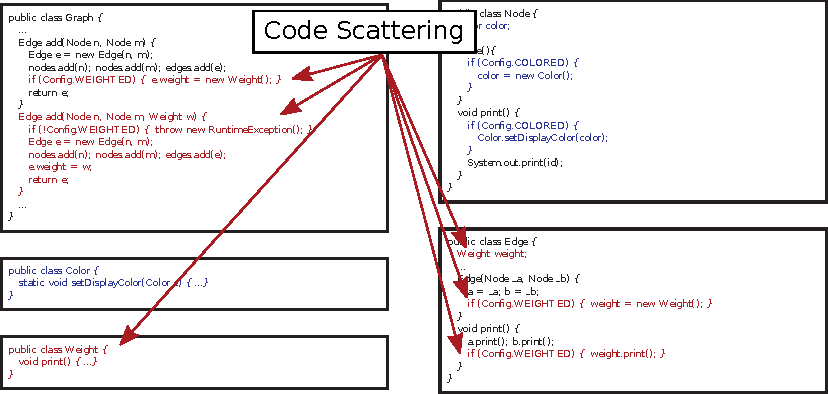
\includegraphics[scale=1.0]{scattering}
	\end{center}
\end{frame}

\subsection{Code Tangling}
\begin{frame}{Problem: Code Tangling}
	\begin{center}
		\vspace{-2mm}
		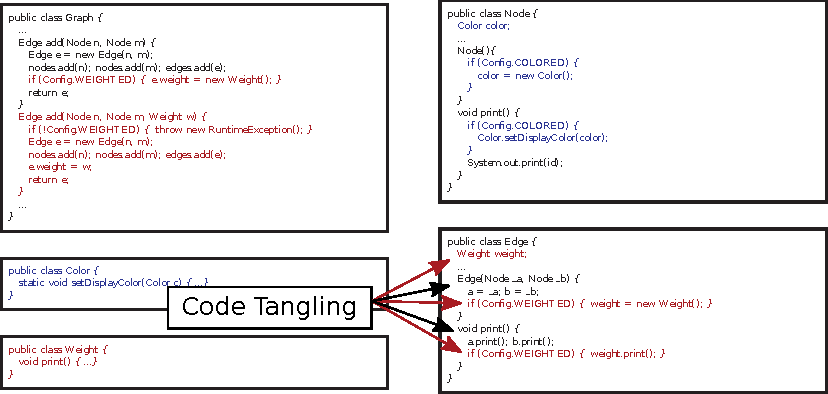
\includegraphics[scale=1.0]{tangling}
	\end{center}
\end{frame}

\subsection{Code Replication}
\begin{frame}{Problem: Code Replication}
	\begin{center}
		\vspace{-2mm}
		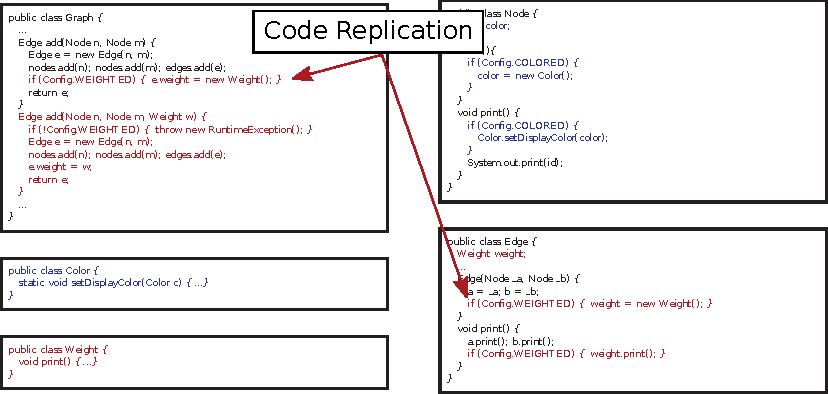
\includegraphics[scale=1.0]{replication}
	\end{center}
\end{frame}

\lessonslearned{
	\item Global (immutable) variables or (lengthy) parameter lists.
	\item Reconfiguration at runtime is possible (in principle).
	\item Variability is spread over the entire program.
	\item Variable parts are always delivered.
		%\begin{itemize}
			%\item Affects code size, resource consumption, performance, ...
			%\item Unused functionality may be risky (security, business strategy, ...)
		%\end{itemize}
}{
	\item \fospl, Chapter 4.
 	\item \featureide, Chapter 17.1.
	%\item P. Hodgson. Feature Toggles. \url{https://martinfowler.com/articles/feature-toggles.html} (TODO: Talk about feature toggles in this lecture?)
}{
	\begin{itemize}
		\item What are the problems with code scattering, tangling and replication?
		\item What are the problems of variable parts being always delivered?
	\end{itemize}
}

\sectionend

\section{Design Patterns for Variability}

% TODO several class diagrams shown here seem to be pixel graphics and should be replaced by vectorized ones

\subsection{Recap on Object-Orientation and Design Patterns}

\begin{frame}{Recap: Object Orientation}
	\begin{mycolumns}[height=50mm]
		\begin{definition}{Key Concepts}
			\begin{itemize}
				\item \textbf{Encapsulation}:\\abstraction and information hiding
				\item \textbf{Composition}:\\nested objects
				\item \textbf{Message Passing}:\\delegating responsibility
				\item \textbf{Distribution of Responsibility}:\\separation of concerns
				\item \textbf{Inheritance}:\\conceptual hierarchy, polymorphism, reuse
			\end{itemize}
		\end{definition}
	\mynextcolumn
		\picDark[width=\linewidth]{oo-concepts-illustration} % TODO what illustrates which concept? why is square not a rectangle or rectangle not a square?
	\end{mycolumns}
\end{frame}

\begin{frame}{Recap: Design Patterns\ \mytitlesource{\gof}}
	\begin{mycolumns}[widths={60}]
		\begin{definition}{Design patterns \deutsch{Entwurfsmuster}}
			\begin{itemize}
				\item Document common solutions to concrete yet frequently occurring design problems
				\item Suggest a concrete implementation for a specific object-oriented programming problem
			\end{itemize}
		\end{definition}	
		\begin{note}{Design Patterns for Variability}
			Many Gang of Four (GoF) design patterns for designing software around stable abstractions and interchangeable (i.e., variable) parts, e.g.
			\begin{itemize}
				\item Template Method
				\item Abstract Factory
				\item Decorator
			\end{itemize}
		\end{note}
	\mynextcolumn
		\picborder{\pic[width=\linewidth]{gof}}
	\end{mycolumns}
\end{frame}

\subsection{Template Method Pattern}
\begin{frame}{\myframetitle}
	\begin{mycolumns}[widths={40}]
		\begin{definition}{Template Method \mysource{\gof\mypages{325--330}}}
			\begin{itemize}
				\item {\bf Intent:} \mycite{Define the overall structure of an algorithm, while allowing subclasses to refine, or redefine, certain steps.}
				\item {\bf Motivation:}  Avoid code replication by implementing the general workflow of an algorithm once, while allowing for necessary variations.
				\item {\bf Idea:} A template method defines the skeleton of an algorithm. Concrete methods override the hook methods.
			\end{itemize}
		\end{definition}
	\mynextcolumn
		\picDark[width=\linewidth]{templatemethod}
	\end{mycolumns}
\end{frame}

\subsection{Abstract Factory Pattern}
\begin{frame}{\myframetitle}
	\begin{mycolumns}[widths={40}]
		\begin{definition}{Abstract Factory \mysource{\gof\mypages{87--95}}}
			\begin{itemize}
				\item {\bf Intent:} \mycite{Provide an interface for creating families of related or dependent objects without specifying their concrete classes.}
				\item {\bf Motivation:} Avoid case distinctions when creating objects of certain kind, consistently create objects of a particular kind.
				\item {\bf Idea:} Create classes for the consistent creation of objects.
			\end{itemize}
		\end{definition}
	\mynextcolumn
		\pic[width=\linewidth]{abstractfactory} % TODO not readible in dark mode
	\end{mycolumns}
\end{frame}

\subsection{Decorator Pattern}
\begin{frame}{\myframetitle}
	\begin{mycolumns}[widths={40}]
		\begin{definition}{Decorator \mysource{\gof\mypages{175--184}}}
			\begin{itemize}
				\item {\bf Intent:} \mycite{Attach additional responsibilities to an object dynamically. Decorators provide a flexible alternative to subclassing for extending functionality.}
				\item {\bf Motivation:} Avoid explosion of static classes when combining all additional behaviors with all applicable classes.
				\item {\bf Idea:} Create decorators and components with the same interface, whereas decorators forward behavior whenever feasible.
			\end{itemize}
		\end{definition}
	\mynextcolumn
		\picDark[width=\linewidth]{decorator}
	\end{mycolumns}
\end{frame}

\subsection{Trade-Offs and Limitations}

\begin{frame}{Object-Oriented Design of our Graph Library}
	\begin{mycolumns}[widths={40}]
		\picDark[width=\linewidth]{graphlib-oo-node-edge}
	\mynextcolumn
		\picDark[width=\linewidth]{graphlib-oo-graph}
	\end{mycolumns}
\end{frame}

\begin{frame}[fragile]{Instantiation Through Template Method Pattern}
	\small
	\begin{mycolumns}[widths={45}]
\begin{codetight}{}
class Graph {
	...
	Edge add(Node n, Node m) {
		Edge e = createEdge();
		nv.add(n); nv.add(m); ev.add(e);
		return e;
	}
	// hook method (with default implementation)
	Edge createEdge(Node n, Node m) {
		return new Edge(n, m);
	}
}
\end{codetight}
\begin{codetight}{}
@class WeightedGraph extends Graph {
	...
	// override hook method
	Edge createEdge(Node n, Node m) {
		Edge e = new WeightedEdge(n, m);
		e.weight = new Weight();
		return e;
	}
}@
\end{codetight}
	\mynextcolumn
		\centering\picDark[width=.7\linewidth]{graphlib-oo-node-edge}
	\end{mycolumns}
\end{frame}

\begin{frame}[fragile]{Instantiation Through Abstract Factory Pattern}
	\small
	\begin{mycolumns}[b]
\begin{codetight}{}
class Graph {
	EdgeFactory edgeFactory;
	...
	Graph(EdgeFactory edgeFactory) {
		this.edgeFactory = edgeFactory;
	}
	Edge add(Node n, Node m) {
		Edge e = edgeFactory.createEdge(n, m);
		nodes.add(n); nodes.add(m); edges.add(e);
		return e;
	}
}
\end{codetight}
\begin{codetight}{}
class EdgeFactory {
	Edge createEdge(Node a, Node b) {
		return new Edge(a, b);
	}
}
\end{codetight}
	\mynextcolumn
		\centering\picDark[width=.75\linewidth]{graphlib-oo-node-edge}	
\begin{codetight}{}
@class WeightedEdgeFactory extends EdgeFactory {
	Edge createEdge(Node a, Node b) {
		Edge e = new WeightedEdge(n, m);
		e.weight = new Weight();
		return e;
	}
}@
\end{codetight}
	\end{mycolumns}
\end{frame}

\begin{frame}{Feature Combinations?}
	\centering\picDark[width=.5\linewidth]{graphlib-oo-diamond}
\end{frame}

\begin{frame}{Diamond Problem}
	\begin{mycolumns}
		\begin{note}{Multiple Inheritance}
			\begin{itemize}
				\item most object-oriented programming languages do not support multiple inheritance (or only provide workarounds)
				\item critical: how to handle name clashes
			\end{itemize}
			% TODO add quote on multiple inheritance?
			% Multiple Inheritance is like a parachute. You don't often need it, but when you do, you really need it. Grady Booch? this one does not really fit here
		\end{note}
	\mynextcolumn
		\picDark[width=\linewidth]{graphlib-oo-diamond-commented}
	\end{mycolumns}
\end{frame}

\begin{frame}{Static Modeling of Feature Combinations}
	\begin{mycolumns}[columns=3,widths={10,80},animation=none]
	\mynextcolumn
		\picDark[width=\linewidth]{graphlib-oo-combinatorial}
		\mynote{}{
			Even if multiple inheritance is supported, statically combining features through inheritance is tedious (or infeasible).
		}
	\mynextcolumn
	\end{mycolumns}
\end{frame}

\begin{frame}[fragile]{Decorator Pattern as a Solution?} % TODO motivation too short
	\begin{mycolumns}[widths={52}]
		\small
\begin{codetight}{}
abstract class GraphDecorator implements IGraph {
	IGraph graph;
	GraphDecorator(IGraph graph) {
		this.graph = graph;
	}
}
\end{codetight}
\begin{codetight}{}
@class WeightedGraph extends GraphDecorator {
	WeightedGraph(IGraph graph) {
		super(graph);
	}
	Edge add(Node n, Node m) {
		WeightedEdge e = (WeightedEdge) graph.add(n, m);
		e.weight = new Weight();
		return e;
	}
	...
}@
\end{codetight} % TODO old slides had a further example. add it?
	\mynextcolumn
		\picDark[width=\linewidth]{graphlib-oo-decorator}
	\end{mycolumns}
	\small
\begin{codetight}{Example Usage}
IGraph graph = @new WeightedGraph(@~new ColoredGraph(~new Graph(@new WeightedEdgeFactory()@)~)~@)@;
\end{codetight}
\end{frame}

\begin{frame}{Delegation Instead of Inheritance}
	\begin{mycolumns}[widths={55}]
		\begin{note}{Discussion}
			Extensions (i.e., features) can be combined dynamically, but \ldots
			\begin{itemize}
				\item must be independent of each other
				\item cannot add public methods
				\item runtime overhead due to indirections
				\item several physical objects are forming a conceptual one (e.g., problems with object identity)
			\end{itemize}
		\end{note}
	\mynextcolumn
		\picDark[width=\linewidth]{graphlib-oo-decorator}
	\end{mycolumns}
\end{frame}


\lessonslearned{
	\item Variability through object-orientation and design patterns
	\item Extension through delegation vs.\ inheritance  
	\item Limitations and drawbacks w.r.t.\ feature combinations
}{
	\item B. Meyer, Object-Oriented Software Construction, Prentice Hall, 1997. Chapters 3, 4
	\item E. Gamma, R. Helm, R. Johnson, and J. Vlissides. Design Patterns: Elements of Reusable Object-Oriented Software. Addison-Wesley, 1995.
}{
	\begin{itemize}
		\item What characterizes a modular software design and why can it support variability?
		\item In which sense are object-oriented solutions more modular than simple conditional statements?
		\item Do you know of other design patterns supporting variability?
	\end{itemize}
}

\sectionend

\mode<beamer>{
	\begin{frame}{\inserttitle}
		\lectureseriesoverview
	\end{frame}

	\contentoverview
}


\end{document}
